
\PassOptionsToPackage{hyphens}{url}

\documentclass[
	usenames,
	dvipsnames,
	handout
] {beamer}

\usepackage{bold-extra}		% Gives us bold tt font.
\usepackage{changepage}
\usepackage{enumitem}
\usepackage{hyperref}
\usepackage{ifthen}
\usepackage{listings}
\usepackage{tikz}

\usetheme[outer/progressbar=foot]{metropolis}

\usetikzlibrary{positioning}

\lstset{
	language=R,
	basicstyle=\ttfamily\small,
	breaklines=true,
	rulecolor=\color{black},
	tabsize=2,
	keywordstyle=\color{RoyalBlue},
	upquote=true,
	otherkeywords={::},
	commentstyle=\color{red},
	stringstyle=\color{ForestGreen}
}

\hypersetup{colorlinks=true, urlcolor=blue, linkcolor=.}

\newcommand{\kw}[1]{\textcolor{blue}{#1}}
\newcommand{\fun}[1]{\textcolor{brown}{#1}}

% Regex elements
\newcommand{\reDigit}{\textbackslash{}d}
\newcommand{\reNonDigit}{\textbackslash{}D}
\newcommand{\reWord}{\textbackslash{}w}
\newcommand{\reSpace}{\textbackslash{}s}
\newcommand{\reNewLine}{\textbackslash{}n}

\newcommand{\rePattern}[1]{{\Large\texttt{\textcolor{blue}{#1}}}}
\newcommand{\reMatch}[1]{\texttt{\textcolor{blue}{#1}}}
\newcommand{\reNoMatch}[1]{\texttt{\textcolor{red}{#1}}}


\title{Intro to Regular Expressions}
\author{Richard Mills}
\date{}


\begin{document}
\maketitle

\begin{frame}{Outline}
	\tableofcontents
\end{frame}
				
\section{Introduction}
\begin{frame}{What are regular expressions?}
	\begin{itemize}[label=\textbullet]
		\item Also known as \textit{regex}.
		      \pause
		\item The concept dates back to the 1950s.
			\pause
		\item A sequence of characters that define a search \textit{pattern} for text.
		      \pause
		\item Frequently used for:
		      	\begin{itemize}[label=\textendash]
			      	\item Checking to see if part/all of a string meets some criteria.
			      	      \pause
			      	\item Perform (advanced) find-and-replace operations within a string.
			      	      \pause
			      	\item Commonly used in compilers/interpreters for parsing user code.
			      	      \pause
			      	\item Input validation for websites.
			      		\pause
				\item Frankly... Useful any time when working with text data!
		      	\end{itemize}
	\end{itemize}
\end{frame}

\begin{frame}{Wildcards}
	\begin{itemize}[label=\textbullet]
		\item Certain Excel formulae allow the use of \textit{wildcards} (ie. regex-lite) when matching against text.
		      \pause

		      \begin{itemize}[label=\textendash]
			      	\item Count number of strings with only 3 characters:\\
			      	      \hfill\texttt{=COUNTIF(A1:A100, "???")}
			      	      \medskip
			      	      \pause
			      	\item Count all strings beginning with \texttt{ABC}:\\
			      	      \hfill\texttt{=COUNTIF(A1:A100, "ABC*")}
			      	      \medskip
			      	      \pause
			      	\item \texttt{?} represents any single character.
			      	      \pause
			      	\item \texttt{*} represents zero or more of any character.
			      		\pause
		      \end{itemize}
		      \medskip
		      
		\item Other supporting functions include \texttt{MATCH}, \texttt{VLOOKUP}, \texttt{SUMIF} and \texttt{SUMIFS}.
			\pause
		      \medskip		      
		\item There is similar functionality in Access via the \texttt{LIKE} operator.
		      \pause
		      \begin{itemize}
		      		\item For example... \hfill\texttt{TABLE\_NUMBER IS LIKE "73?"}
		      \end{itemize}
	\end{itemize}
\end{frame}
  
\section{Working with file-names}
\begin{frame}{What's the issue?}
	\begin{itemize}[label=\textbullet]
		\item<1-> Suppose we have the following files within a folder: \\
			\medskip
			\begin{itemize}
				\item<2-> \texttt{TOP\_SECRET\_DATA\_\textcolor<3->{orange}{01-03-2020}.CSV}
				\item<2-> \texttt{TOP\_SECRET\_DATA\_\textcolor<3->{orange}{20-03-2020}.CSV}
				\item<2-> \texttt{TOP\_SECRET\_DATA\_\textcolor<3->{orange}{25-04-2020}.CSV}
			\end{itemize}
		\item<3-> The date within the file-name gives us the effective date of the data within.
		\item<4-> \textbf{How could we extract those dates?}
	\end{itemize}
\end{frame}
    
\begin{frame}{What's the issue?}
	\begin{itemize}[label=\textbullet]
		\item \textbf{What about now?} \\
		      \medskip
		      \begin{itemize}
			      	\item \texttt{TOP\_SECRET\_DATA\_\textcolor{orange}{01-03-2020}.CSV}
			      	\item \texttt{TOP\_SECRET\_DATA\_V2\_\textcolor{orange}{20-03-2020}.CSV}
			      	\item \texttt{TOP\_SECRET\_DATA\_Adj\_\textcolor{orange}{25-04-2020}.CSV}
		      \end{itemize}
	\end{itemize}
\end{frame}
    
\begin{frame}{Possible solution}
	If we were \textit{particularly} determined, we could use the following pseudo-code: \\
		\pause
	\medskip
		
	\begin{ttfamily}
		\begin{tabbing}
			\small
			--\=--\=--\=--\=--\=--\=\kill
			\kw{for} i \kw{from} 1 \kw{to} LEN(string)-10: \\
				\pause
			\> \kw{if} \fun{is\_digit}(string[i]) \kw{and} \fun{is\_digit}(string[i+1]): \\
				\pause
			\>\> \kw{if} string[i+2] = "-": \\
				\pause
			\>\>\> \kw{if} \fun{is\_digit}(string[i+3]) \kw{and} \fun{is\_digit}(string[i+4]): \\
				\pause
			\>\>\>\> \kw{if} string[i+5] = "-": \\
				\pause
			\>\>\>\>\> \kw{if} \fun{is\_digit}(string[i+6]) .... : \\
				\pause
			\>\>\>\>\>\> date\_part = string[i:i+10] \\
				\pause
			\>\>\>\>\>\> \kw{return} date\_part \\[1em]
				\pause
			\kw{error} `No date!'
				\pause
		\end{tabbing}
	\end{ttfamily}
	
	\medskip
	\textbf{Is there an alternative way?}
\end{frame}
    
\begin{frame}{Possible solution}
	\begin{itemize}[label=\textbullet]
		\item In \textit{regex speak} we are looking for the following pattern: \\
		      \bigskip
		      \hspace*{3em}
		      \rePattern{\reDigit\reDigit-\reDigit\reDigit-\reDigit\reDigit\reDigit\reDigit}
				\pause
		      \bigskip		      
		\item Where each \rePattern{\reDigit} corresponds to a single digit (0-9).
		      \pause
		\item This would match any of the dates contained within the above file names.
		      \pause
		\item However, it \textit{could} leave to false positives, eg:
		      \begin{itemize}[label=\textendash]
			      	\item \texttt{RANDOM\_\textcolor{orange}{00-01-0002}.CSV}
			      	      \pause
			      	\item \texttt{12\textcolor{orange}{34-56-7890}1234.CSV}
			      		\pause
		      \end{itemize}		      
		\item \textbf{Can we refine it?}
	\end{itemize}
\end{frame}
    
\begin{frame}{Possible solution}
	\begin{itemize}[label=\textbullet]
		\item Previously we used \rePattern{\reDigit} to match a single digit.
		      \pause
		\item We could instead use a \textbf{character class} to restrict this behaviour.
		      \pause
		\item This allows us to specify a list (or range) of permitted characters.
		      \pause
		\item As an example, we'll assume that:
		      \pause
		      \begin{itemize}[label=\textendash]
			      	\item The \textit{day} part can start with any of \texttt{0}, \texttt{1}, \texttt{2} or \texttt{3}.
			      	      \pause
			      	\item The \textit{month} part can start with either \texttt{0} or \texttt{1}.
			      	      \pause
			      	\item The \textit{year} part will start with either \texttt{19} or \texttt{20}.
			      		\pause
		      \end{itemize}		      
		      \bigskip
		\item We can update our pattern to be: \\
		      \bigskip
		      \hspace*{3em}
		      \rePattern{\underline{[0-3]}\reDigit-\underline{[01]}\reDigit-\underline{(19$|$20)}\reDigit\reDigit}
	\end{itemize}
\end{frame}

\begin{frame}{Possible solution}
	\hspace*{3em}
	\rePattern{[0-3]\reDigit-[01]\reDigit-(19$|$20)\reDigit\reDigit}
	\pause
	\bigskip
	
	\begin{itemize}[label=\textbullet]
		\item Note the use of the following elements: \\
		      \pause
		      \medskip
		      \begin{itemize}[label=\textendash]
			      	\item \rePattern{[0-3]} which matches against any of \texttt{0}, \texttt{1}, \texttt{2} or \texttt{3}. \\
			      	      \pause
			      	      \medskip
			      	\item \rePattern{[01]} which matches either \texttt{0} or \texttt{1}. \\
			      	      \pause
			      	      \medskip
			      	\item \rePattern{(19$|$20)} which matches either \texttt{19} or \texttt{20}. \\
					\begin{itemize}
						\item [] \footnotesize Note the use of \rePattern{(} and \rePattern{)} above.
			      		\end{itemize}
		      \end{itemize} 
	\end{itemize}  
\end{frame}
    
\begin{frame}{Possible solution}
	\hspace*{3em}
	\rePattern{[0-3]\reDigit-[01]\reDigit-(19$|$20)\reDigit\reDigit}
		\pause
	\bigskip

	\begin{itemize}[label=\textbullet]
		\item Note the 2x \rePattern{\reDigit} at the end.
		      \pause
		\item We could instead use a \textbf{quantifier} to remove duplication: \\
		      \bigskip
		      \hspace*{3em}
		      \rePattern{[0-3]\reDigit-[01]\reDigit-(19$|$20)\reDigit\underline{\{2\}}}
		      		\pause
		      \bigskip
		\item Both approaches are equivalent!
	\end{itemize}  
\end{frame}
    
\begin{frame}{Possible solution}
	\hspace*{3em}
	\rePattern{[0-3]\reDigit-[01]\reDigit-(19$|$20)\reDigit\{2\}}
		\pause
	\bigskip	
	\begin{itemize}[label=\textbullet]
		\item \textbf{What if the day and month components didn't always have a leading 0?}
		      \pause
		      \begin{itemize}[label=\textendash]
			      	\item \texttt{TOP\_SECRET\_DATA\_\textcolor{orange}{1-03-2020}.CSV}
			      	\item \texttt{TOP\_SECRET\_DATA\_V2\_\textcolor{orange}{20-3-2020}.CSV}
			      	\item \texttt{TOP\_SECRET\_DATA\_Adj\_\textcolor{orange}{5-4-2020}.CSV}
		      \end{itemize}
		      		\pause
		      \bigskip
		\item We could use \rePattern{?} which is another type of quantifier. \\
			\pause
		      \medskip		      
		      \begin{itemize}[label=\textendash]
		      		\item This matches the prior element 0 \textbf{or} 1 times.		      			
		      \end{itemize}
		      		\pause	      		      
	\end{itemize}
	
	\bigskip
      \hspace*{3em}
      \rePattern{[0-3]\underline{?}\reDigit-[01]\underline{?}\reDigit-(19$|$20)\reDigit\{2\}}
\end{frame}
    
\begin{frame}{Possible solution}
	\begin{itemize}[label=\textbullet]
		\item The last change we \textit{might} want to make is to ensure that either end of a potential date does \textbf{not} touch a digit.
		      \pause
		\item For this, we can use:
		      \pause
		      \begin{itemize}[label=\textendash]
			      	\item \rePattern{\reNonDigit} to match a \underline{non}-digit character. \\
					\pause
			      	      \medskip			      	      
			      	\item {\Large\textcolor{blue}{(?\textless=...)}} to match an element immediately \underline{preceding} our date. \\
					\pause
			      	      \medskip			      	      
			      	\item {\Large\textcolor{blue}{(?=...)}} to match an element immediately \underline{after} our date. \\
			      		\pause
			      	      \medskip			      	      
		      \end{itemize}
		\item Our final proposed pattern is: \\
		      \bigskip
	\end{itemize}
	
	\rePattern{\underline{(?\textless=\reNonDigit)}[0-3]?\reDigit-[01]?\reDigit-(19$|$20)\reDigit\{2\}\underline{(?=\reNonDigit)}}
\end{frame}

\begin{frame}{Possible solution}
	
	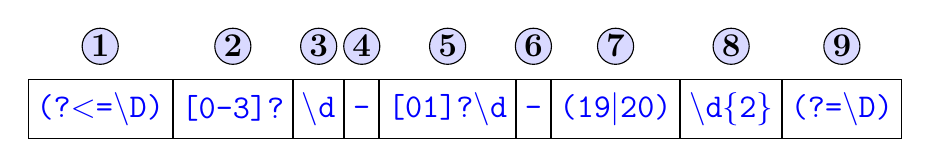
\begin{tikzpicture}[node distance=0]
		
		\def \elements {(?\textless=\reNonDigit),[0-3]?,\reDigit,-,[01]?\reDigit,-,(19$|$20),\reDigit\{2\},(?=\reNonDigit)}
					
		\tikzset{element/.style={thin, minimum height=0.75cm, inner xsep=3pt, text=blue}};
					
		\tikzset{idxLabel/.style={shape=circle, inner sep=1pt, fill=blue!15}};
					
		\foreach \element [count=\idx] in \elements {
			\ifthenelse{\idx = 1} {
				\node[draw, element] (\idx) {\texttt{\large \element}};			
			} {
				\node[draw, element, right=of \the\numexpr\idx-1\relax] (\idx) {\texttt{\large \element}};
			}
					
			\node [draw, idxLabel, above=5pt of \idx] {\textbf{\large \idx}};
		}
					
	\end{tikzpicture}

	\begin{itemize}[leftmargin=0pt]
			\pause
		\item[1] The character immediately before our date must be a \underline{non}-digit
			\pause
		\item[2] The \textbf{day} part must start with an optional \texttt{0}, \texttt{1}, \texttt{2} or \texttt{3}
			\pause
		\item[3] \ldots followed by a \texttt{0}--\texttt{9}
			\pause
		\item[4] \ldots followed by a --
			\pause
		\item[5] \ldots followed by the \textbf{month} part which can start with an optional \texttt{0} or \texttt{1}
			\pause
		\item[6] \ldots followed by a --
			\pause
		\item[7] \ldots followed by the \textbf{year} part which must start with \texttt{19} or \texttt{20}
			\pause
		\item[8] \ldots followed by 2x digits
			\pause
		\item[9] The character immediately after our date must be a \underline{non}-digit
	\end{itemize}
					
\end{frame}

\begin{frame}{Possible solution}

	Below shows the `evolution' of our pattern: \\
	\bigskip
	
	\rePattern{\reDigit\reDigit-\reDigit\reDigit-\reDigit\reDigit\reDigit\reDigit} \\
		\pause
	\bigskip
	
	\rePattern{\underline{[0-3]}\reDigit-\underline{[01]}\reDigit-\underline{(19$|$20)}\reDigit\reDigit} \\
	      	\pause
	\bigskip
	      		
	\rePattern{[0-3]\reDigit-[01]\reDigit-(19$|$20)\underline{\reDigit\{2\}}} \\
	      	\pause
	\bigskip
      
      \rePattern{[0-3]\underline{?}\reDigit-[01]\underline{?}\reDigit-(19$|$20)\reDigit\{2\}} \\
		\pause
	\bigskip
	
	\rePattern{\underline{(?\textless=\reNonDigit)}[0-3]?\reDigit-[01]?\reDigit-(19$|$20)\reDigit\{2\}\underline{(?=\reNonDigit)}} \\
\end{frame}
    
\begin{frame}{Possible solution}
	\rePattern{(?\textless=\reNonDigit)[0-3]?\reDigit-[01]?\reDigit-(19$|$20)\reDigit\{2\}(?=\reNonDigit)}
		\pause
		
	\medskip
	\begin{itemize}[label=\textbullet]
		\item This pattern will successfully match against (for example):
		      \pause
		      \begin{itemize}[label=\textendash]
		      	\item \texttt{TOP\_SECRET\_DATA\_\textbf{\textcolor{SeaGreen}{01-03-2020}}.CSV}
		      	      \pause
		      	\item \texttt{TOP\_SECRET\_DATA\_\textbf{\textcolor{SeaGreen}{1-03-2020}}.CSV}
		      	      \pause
		      	\item \texttt{TOP\_SECRET\_DATA\_V2\_\textbf{\textcolor{SeaGreen}{20-3-2020}}.CSV}
		      	      \pause
		      	\item \texttt{TOP\_SECRET\_DATA\_\textbf{\textcolor{SeaGreen}{5-4-1999}}\_Adj.CSV}
		      \end{itemize}
	\end{itemize}
\end{frame}

\begin{frame}{Possible solution}
	\rePattern{(?\textless=\reNonDigit)[0-3]?\reDigit-[01]?\reDigit-(19$|$20)\reDigit\{2\}(?=\reNonDigit)}
	\medskip
	
	\begin{itemize}[label=\textbullet]
		\item Given the above pattern... \textbf{Which of the following would be successfully matched?}
		      \begin{itemize}[label=\textendash]
				\item<2-> \texttt{\textbf<3->{\textcolor<3->{red}{OUR\_DATA\_FILE\_01-03-2120.CSV}}}
			      	\item<4-> \texttt{SKETCHY\_INPUTS\_V\textbf<5->{\textcolor<5->{SeaGreen}{31-10-1999}}.CSV}
			      	\item<6-> \texttt{\textbf<7->{\textcolor<7->{red}{20-10-1999\_NO\_PEEKING.TXT}}}
			      	\item<8-> \texttt{\textbf<9->{\textcolor<9->{red}{NO10\_PARTY\_INVITES\_31\_10\_1999.CSV}}}
		      \end{itemize}
	\end{itemize}
\end{frame}

\section{Using patterns within code}
\begin{frame}{How do we actually \emph{use} this pattern?}
	\begin{itemize}[label=\textbullet]
		\item Many programming languages provide \emph{Regex} functionality.
			\pause
		\begin{itemize}[label=\textendash]
			\item In VBA via the \texttt{Microsoft VBScript Regular Expressions 5.5} reference.
				\pause
			\item In Python via the \texttt{re} library.
				\pause
			\item In R via the \texttt{stringr} library.
				\pause
		\end{itemize}			
			
		\item However, there \emph{may} be some differences in the respective implementations.
	\end{itemize}
\end{frame}

\begin{frame}{How could we do this within R?}
	\begin{itemize}[label=\textbullet]
		\item Suppose we have some \texttt{.CSV} files within a folder.
			\pause
		\item Let's assume that the variable \texttt{FOLDER\_PATH} contains the path.
			\pause
		\item Within our code, we can list all of the files in the folder...
			\pause
		\item ...and then extract the dates from those files with a valid file name.
	\end{itemize}
\end{frame}

\begin{frame}[fragile]{A worked example in R}
	\begin{adjustwidth}{-1.5em}{-1.5em}
		\begin{lstlisting}
tibble::tibble(
  FILE_NAME =
    fs::dir_ls(
      path = FOLDER_PATH,
      regexp = '(?i)CSV$'  # ...another pattern!
    ),
  
  DATE_PART =
    stringr::str_extract(
      FILE_NAME,
      pattern =
'(?<=\\D)[0-3]?\\d-[01]?\\d-(19|20)\\d{2}(?=\\D)'
    )
)
		\end{lstlisting}
	\end{adjustwidth}
\end{frame}

\begin{frame}{A worked example in R}
	Suppose our folder contained the following files:
	\begin{ttfamily}
		\begin{itemize}[label={}]		
			\item 20\_10\_1999\_NO\_PEEKING.CSV
			\item NO10\_PARTY\_INVITES\_31-10\_1999.CSV
			\item OUR\_DATA\_FILE\_01-03-2120.\underline{csv}
			\item SKETCHY\_INPUTS\_V31-10-1999.CSV
			\item TOP\_SECRET\_DATA\_01-03-2020.CSV
			\item TOP\_SECRET\_DATA\_1-03-2020.CSV
			\item TOP\_SECRET\_DATA\_5-4-1999\_Adj.CSV
			\item TOP\_SECRET\_DATA\_V2\_20-3-2020.CSV
			\item \textcolor{red}{NOT\_A\_CSV.TXT}
		\end{itemize}
	\end{ttfamily}
\end{frame}
		
\begin{frame}{A worked example in R}
	Below shows the output from our code on the above folder: \\
	\medskip
	\begin{center}
		\begin{tabular}{l c}
			\textbf{FILE\_NAME} & \textbf{DATE\_PART} \\	
			20\_10\_1999\_NO\_PEEKING.CSV & \textcolor{red}{NA} \\
			NO10\_PARTY\_INVITES\_31-10\_1999.CSV & \textcolor{red}{NA} \\
			OUR\_DATA\_FILE\_01-03-2120.csv & \textcolor{red}{NA} \\
			SKETCHY\_INPUTS\_V31-10-1999.CSV & 31-10-1999 \\
			TOP\_SECRET\_DATA\_01-03-2020.CSV & 01-03-2020 \\
			TOP\_SECRET\_DATA\_1-03-2020.CSV & 1-03-2020 \\
			TOP\_SECRET\_DATA\_5-4-1999\_Adj.CSV & 5-4-1999 \\
			TOP\_SECRET\_DATA\_V2\_20-3-2020.CSV & 20-3-2020
		\end{tabular}
	\end{center}
\end{frame}

\begin{frame}[fragile]{A worked example in R}
	\begin{itemize}[label=\textbullet]
		\item If we \emph{pipe} our \texttt{DATE\_PART} into \texttt{lubridate::dmy}, we can convert our extracted date into an actual date object that we can more easily work with.
			\pause
		\item We can also use \texttt{dplyr::filter} to only retain those file names with valid dates.
			\pause
	\end{itemize}

	\medskip
		
	\begin{lstlisting}
tibble::tibble(
  ...
  DATE_PART =
    ... %>%
    lubridate::dmy()    
) %>%
dplyr::filter(
  !is.na(DATE_PART)
)
	\end{lstlisting}
\end{frame}

\begin{frame}{A worked example in R}
	Our revised output is shown below: \\
	\medskip
	\begin{center}
		\begin{tabular}{l c}
			\textbf{FILE\_NAME} & \textbf{DATE\_PART} \\	
			SKETCHY\_INPUTS\_V31-10-1999.CSV & 1999-10-31 \\
			TOP\_SECRET\_DATA\_01-03-2020.CSV & 2020-03-01 \\
			TOP\_SECRET\_DATA\_1-03-2020.CSV & 2020-03-01 \\
			TOP\_SECRET\_DATA\_5-4-1999\_Adj.CSV & 1999-04-05 \\
			TOP\_SECRET\_DATA\_V2\_20-3-2020.CSV & 2020-03-20
		\end{tabular}
	\end{center}
\end{frame}

\section{Wrap up}
\begin{frame}{What can I take away from this?}
	\begin{itemize}[label=\textbullet]
		\item That regex patterns can be used to match characters within some wider text.
			\pause
		\item Using various elements within our pattern, we can refine what we are looking for.
			\pause
		\item We are not just restricted to numbers!
	\end{itemize}
\end{frame}

\begin{frame}{What didn't we see?}
	\begin{itemize}[label=\textbullet]
		\item In our example above, we could have used \emph{capture groups} to extract the individual day, month and year parts.
			\pause
		\item ...these can also be used to make a pattern dependent on what has already been matched.
			\pause
		\item Additional \emph{quantifiers} such as \rePattern{+} and \rePattern{*}.
			\pause
		\item Using \emph{anchors} such as \rePattern{\^{}} and \rePattern{\$} to ensure that matches begin and/or finish at the start/end of a string respectively.
			\pause
		\item Many other character classes such as \rePattern{\reWord}, \rePattern{\reSpace} and \rePattern{\reNewLine}.
			\pause
		\item \emph{Flags}; for example \rePattern{(?i)} makes a pattern case-insensitive.
	\end{itemize}
\end{frame}

\begin{frame}{Useful resources}
	For those wanting to know more: \\
		\pause
	\medskip

	\begin{itemize}[label=\textbullet]
		\item \url{https://regexone.com/}
			\pause
		\item \url{https://unicode-org.github.io/icu/userguide/strings/regexp.html}
			\pause
		\item \url{https://medium.com/factory-mind/regex-tutorial-a-simple-cheatsheet-by-examples-649dc1c3f285}
			\pause
		\item Speak to me.
	\end{itemize}
\end{frame}

\begin{frame}{That's it!}
	\Huge
	\bfseries
	\begin{center}	
		Any questions?
		
		\ldots comments?
	\end{center}
\end{frame}
			
\end{document}